\documentclass[11pt]{article}

\usepackage[margin=1in]{geometry}
\usepackage{amsmath}
\usepackage{booktabs}
\usepackage{graphicx}
\usepackage{hyperref}
\usepackage{caption}
\usepackage{subcaption}

\title{Migration Shocks as an Instrument for Rent Growth}
\author{Chenyu Gu \and Ocean Wang \and Ike Peng}
\date{May 2026}

\begin{document}
\maketitle

\begin{abstract}
This project studies whether pandemic-era population inflows caused local rent growth. The unit is a U.S. county. The treatment is an increase in county population growth during the migration-shock period, and we use IRS pandemic-era migration shocks as an instrument for that endogenous treatment. The outcome is rent-growth acceleration from Zillow's county Zillow Observed Rent Index. The main IV estimate implies that a one percentage point increase in the population-growth shock raises rent-growth acceleration by 2.33 percentage points, with a 95 percent confidence interval from 0.47 to 4.19 percentage points. The first stage is meaningful: a one percentage point IRS migration shock predicts a 0.69 percentage point increase in the Census population-growth shock, with first-stage $F=13.5$. Results are positive in the no-control and baseline-control specifications, but become smaller and imprecise after adding state fixed effects, so the evidence should be interpreted as suggestive rather than definitive.
\end{abstract}

\section{Introduction}

The expansion of remote work during and after the pandemic changed residential location choices across U.S. counties. Some counties received unusually large inflows, while others experienced little change or outflows. These migration shifts may have increased local housing demand and pushed up rents, especially in places where the rental market could not quickly adjust.

The causal question is: \emph{what is the effect of population-growth shocks on rent-growth acceleration?} The empirical challenge is that population growth is endogenous. Counties attracting new residents may also have improving amenities, stronger labor markets, or rising expectations about future growth. To address this, we use pandemic-era IRS migration shocks as an instrument for actual county population-growth shocks. The instrument captures abnormal migration inflows in 2021--2022 relative to each county's 2019--2020 migration baseline.

The pandemic appears in the analysis as the source of the migration shock, not as the treatment itself. The treatment is the change in county population growth induced by migration; the outcome is rent-growth acceleration. This distinction matters because the goal is not to estimate the total effect of COVID-19 on rents, but to estimate the housing-market effect of population inflows generated during the migration-shock period.

\section{Causal Setup}

The observational unit is a county. Each county has potential rent-growth acceleration under different values of the population-growth shock. A county is more ``treated'' when its population growth rises more in the migration-shock years 2021--2022 relative to its own 2019--2020 baseline. A county is less treated, or effectively untreated, when its population-growth shock is near zero or negative: its population growth did not accelerate relative to the pre-shock period.

Because treatment intensity is continuous, the estimand is not a binary treated-versus-control average treatment effect. It is the causal effect of a one percentage point increase in the county population-growth shock on rent-growth acceleration. Formally, the treatment is
\[
D_c =
\overline{\Delta \log Pop}_{c,2021:2022}
-
\overline{\Delta \log Pop}_{c,2019:2020}.
\]
The outcome is
\[
Y_c =
\overline{\Delta \log Rent}_{c,2021:2022}
-
\overline{\Delta \log Rent}_{c,2019:2020}.
\]

Treatment is endogenous because counties with accelerating population growth may also have rising amenities, labor demand, or housing-market expectations. We therefore use an instrument:
\[
Z_c =
\overline{IRSInflowRate}_{c,2021:2022}
-
\overline{IRSInflowRate}_{c,2019:2020}.
\]
A county receives a larger instrument shock if IRS tax-return migration data show an unusually large increase in domestic inflows during the migration-shock period. The instrument is not the treatment; it is the source of plausibly exogenous variation used to isolate the population-growth component of local housing-demand shocks.

\section{Data}

We use four public county-level data sources. The outcome is annual log rent growth from Zillow's county ZORI file.\footnote{\url{https://www.zillow.com/research/data/}} Monthly ZORI observations are averaged to the county-year level, keeping county-years with at least nine observed months. The instrument comes from IRS SOI county-to-county migration files for 2018--2019, 2019--2020, 2020--2021, and 2021--2022.\footnote{\url{https://www.irs.gov/statistics/soi-tax-stats-migration-data}} These files report domestic migration based on year-to-year address changes in tax returns.

The endogenous treatment is actual population growth from Census county population estimates.\footnote{\url{https://www.census.gov/programs-surveys/popest.html}} We use the 2010--2020 and 2020--2023 county population-estimate files to construct annual log population growth for 2019--2022. We also use Census Building Permits Survey data to control for 2020 residential permits per capita.\footnote{\url{https://www.census.gov/construction/bps/}} Because county-level legal zoning measures are not consistently available for the full sample, we use low 2020 permitting intensity as a proxy for supply constraints in the heterogeneity analysis. The final IV sample contains 542 counties with complete Zillow, IRS, Census population, and permits data.

The time dimension is defined around migration shocks, not around a generic COVID post-period. The pre-shock period is IRS destination years 2019--2020, and the shock period is 2021--2022, when the county migration files capture the main relocation response. Appendix Figure~\ref{fig:timeline} plots rent-growth trends by migration-shock tercile on this migration-year timeline.

\section{Empirical Strategy}

The main estimating equation is
\[
Y_c = \beta D_c + X_c'\gamma + \varepsilon_c,
\]
where $D_c$ is instrumented by $Z_c$. The baseline controls $X_c$ are pre-shock rent growth, log 2020 rent, and 2020 permits per capita. We also report a no-control specification and a more demanding robustness specification with state fixed effects.

The IV assumptions are relevance and exclusion. Relevance means that the IRS migration shock must predict actual county population growth. This is testable in the first stage. Exclusion means that, conditional on controls, the IRS migration shock affects rent acceleration only through local population growth. This would be violated if migration shocks proxy for other simultaneous local demand shocks, such as amenity revaluation or local labor-market booms, that affect rents independently of population growth.

For heterogeneity, we split counties by 2020 residential permits per capita. Below-median permit counties are treated as more supply constrained, while above-median permit counties are treated as less constrained. This is a proxy for zoning restrictiveness rather than a direct legal zoning index.

\section{Population Inflow Effect}

The first stage is strong enough for the baseline design. A one percentage point IRS migration shock predicts a 0.69 percentage point increase in the Census population-growth shock. The robust first-stage $F$ statistic is 13.5. The reduced form is also positive: a one percentage point IRS migration shock predicts a 1.60 percentage point increase in rent-growth acceleration.

The baseline IV estimate is 2.33. Interpreted in percentage-point units, a one percentage point increase in the population-growth shock raises rent-growth acceleration by about 2.33 percentage points. The 95 percent confidence interval is 0.47 to 4.19 percentage points. This magnitude is economically meaningful because the outcome is an acceleration in annual rent growth, not a rent-level change. A county whose population growth increased sharply during the migration-shock period would therefore be predicted to experience a noticeably larger rent-growth acceleration.

Appendix Table~\ref{tab:shockbin} helps interpret the shock groups. High-shock counties have an average IRS migration shock of 0.64 percentage points, compared with -0.12 percentage points for low-shock counties. They also have higher average population-growth shocks and rent acceleration. Appendix Figure~\ref{fig:timeline} shows that the high-shock group does not simply have much higher rent growth in every pre-shock year; the separation becomes clearer in the migration-shock years.

\section{Heterogeneity and Robustness}

The second research question is whether population inflows have larger rent effects in more supply-constrained housing markets. Ideally, this would be tested with a direct county-level zoning restrictiveness measure. Because such measures are not consistently available for the full county sample, we use 2020 residential permits per capita as a proxy for supply constraints. Counties below the sample median in permits per capita are classified as low-permit, more constrained counties; counties above the median are classified as high-permit, less constrained counties.

Appendix Table~\ref{tab:heterogeneity} reports the heterogeneity estimates. The low-permit group has a larger point estimate, 5.37, which is directionally consistent with stronger rent effects in constrained markets. However, this estimate is very imprecise: the confidence interval ranges from -4.96 to 15.69, and the first-stage $F$ statistic is only 1.16. This weak first stage means the low-permit heterogeneity estimate is not reliable. In contrast, the high-permit group has a stronger first stage, with $F=17.77$, and a more precise positive estimate of 2.15. Therefore, the data do not provide robust evidence that the rent effect is larger in more supply-constrained counties.

We also conduct robustness checks by varying the controls in the main IV specification. Appendix Table~\ref{tab:iv} reports three versions: no controls, baseline controls, and baseline controls plus state fixed effects. The no-control estimate is 3.43, while the baseline-control estimate is 2.33. Adding state fixed effects reduces the estimate to 0.60 and makes it statistically imprecise. This pattern suggests that broad regional variation contributes to the main estimate. The sign remains positive across specifications, but the magnitude is not fully robust to absorbing state-level variation.

Taken together, the robustness and heterogeneity results qualify the main population-inflow finding. The baseline IV result supports a positive rent effect of population-growth shocks, but the zoning-related heterogeneity claim is weaker. The most defensible conclusion is that pandemic-era population inflows likely increased rent growth, while evidence that this effect was larger in more supply-constrained markets is suggestive at best.

\section{Discussion}

The evidence is consistent with the view that pandemic-era population inflows raised rent growth in receiving counties. The IV design uses migration shocks as a source of variation in actual county population growth, and the timing is based on the observed migration-shock period rather than on a generic post-COVID indicator. Under the exclusion restriction, the baseline estimate implies an economically meaningful rent response to population-growth shocks.

The main limitation is exclusion. Migration shocks may capture changes in preferences for amenities, climate, or remote-work destinations that affect rents beyond measured population growth. A second limitation is that the state fixed-effect robustness estimate is smaller and imprecise, meaning the strongest variation is regional. We therefore present the result as evidence consistent with a causal effect, not as a fully definitive estimate.

The zoning heterogeneity result should also be interpreted cautiously. Permitting intensity is an imperfect proxy: low permits may reflect restrictive zoning, but it may also reflect weak demand, geography, or administrative differences. The heterogeneity exercise is therefore a supply-constraint robustness check rather than direct evidence on zoning law.

\clearpage
\appendix
\section{Appendix Tables and Figures}

\begin{table}[h!]
\centering
\caption{Summary by IRS Migration-Shock Tercile}
\label{tab:shockbin}
\small
\begin{tabular}{lrrrrr}
\toprule
Shock group & Counties & IRS shock & Pop. shock & Rent accel. & Pre growth \\
\midrule
Low shock & 181 & -0.0012 & 0.0007 & 0.0514 & 0.0401 \\
Medium shock & 180 & 0.0019 & 0.0040 & 0.0532 & 0.0403 \\
High shock & 181 & 0.0064 & 0.0057 & 0.0682 & 0.0412 \\
\bottomrule
\end{tabular}
\caption*{\footnotesize Notes: Shocks are post-period averages for 2021--2022 minus pre-period averages for 2019--2020.}
\end{table}

\begin{table}[h!]
\centering
\caption{IV Estimates}
\label{tab:iv}
\small
\begin{tabular}{lrrrrr}
\toprule
Specification & Estimate & Std. error & 95\% CI low & 95\% CI high & First-stage F \\
\midrule
No controls & 3.433 & 1.524 & 0.446 & 6.420 & 9.113 \\
Baseline controls & 2.330 & 0.947 & 0.473 & 4.187 & 13.514 \\
Controls + state FE & 0.599 & 0.568 & -0.514 & 1.712 & 5.660 \\
\bottomrule
\end{tabular}
\caption*{\footnotesize Notes: The endogenous treatment is the Census population-growth shock. The instrument is the IRS migration shock.}
\end{table}

\begin{table}[h!]
\centering
\caption{First Stage and Reduced Form}
\label{tab:fsrf}
\begin{tabular}{llrrr}
\toprule
Model & Dependent variable & Estimate & Std. error & F-stat \\
\midrule
First stage & Population-growth shock & 0.687 & 0.187 & 13.514 \\
Reduced form & Rent-growth acceleration & 1.601 & 0.351 &  \\
\bottomrule
\end{tabular}
\caption*{\footnotesize Notes: Estimates use the baseline-control specification.}
\end{table}

\begin{table}[h!]
\centering
\caption{Supply-Constraint Heterogeneity}
\label{tab:heterogeneity}
\small
\begin{tabular}{lrrrrr}
\toprule
Group & Estimate & Std. error & 95\% CI low & 95\% CI high & First-stage F \\
\midrule
Low-permit / more constrained & 5.365 & 5.270 & -4.964 & 15.694 & 1.163 \\
High-permit / less constrained & 2.151 & 0.890 & 0.406 & 3.896 & 17.768 \\
\bottomrule
\end{tabular}
\caption*{\footnotesize Notes: Low-permit counties are below the sample median in 2020 residential permits per capita. Estimates use pre-shock rent growth and log 2020 rent controls.}
\end{table}

\begin{table}[h!]
\centering
\caption{Descriptive Statistics}
\label{tab:desc}
\small
\begin{tabular}{lrrrr}
\toprule
Variable & Mean & Std. dev. & Min & Max \\
\midrule
Rent acceleration & 0.0576 & 0.0259 & -0.0063 & 0.2837 \\
Population-growth shock & 0.0035 & 0.0132 & -0.0537 & 0.0816 \\
IRS migration shock & 0.0024 & 0.0039 & -0.0155 & 0.0262 \\
Pre rent growth & 0.0405 & 0.0172 & -0.0639 & 0.1125 \\
2020 permits per capita & 5.5440 & 4.3299 & 0.2153 & 25.4654 \\
\bottomrule
\end{tabular}
\end{table}

\begin{table}[h!]
\centering
\caption{Counties with the Largest IRS Migration Shocks}
\label{tab:top}
\footnotesize
\begin{tabular}{llrrr}
\toprule
County & State & IRS shock & Pop. shock & Rent accel. \\
\midrule
Kaufman County & TX & 0.0262 & 0.0393 & 0.0437 \\
Saint Lucie County & FL & 0.0147 & 0.0056 & 0.1217 \\
Marion County & FL & 0.0136 & 0.0108 & 0.0926 \\
Bay County & FL & 0.0133 & 0.0816 & -0.0019 \\
Polk County & FL & 0.0133 & 0.0028 & 0.0773 \\
Johnson County & TX & 0.0127 & 0.0189 & 0.0564 \\
Lee County & FL & 0.0127 & -0.0034 & 0.1401 \\
Rockwall County & TX & 0.0126 & 0.0136 & 0.0578 \\
Manatee County & FL & 0.0125 & 0.0000 & 0.1306 \\
New York County & NY & 0.0122 & 0.0008 & 0.1013 \\
\bottomrule
\end{tabular}
\end{table}

\begin{figure}[h!]
\centering
\begin{subfigure}{0.49\linewidth}
  \centering
  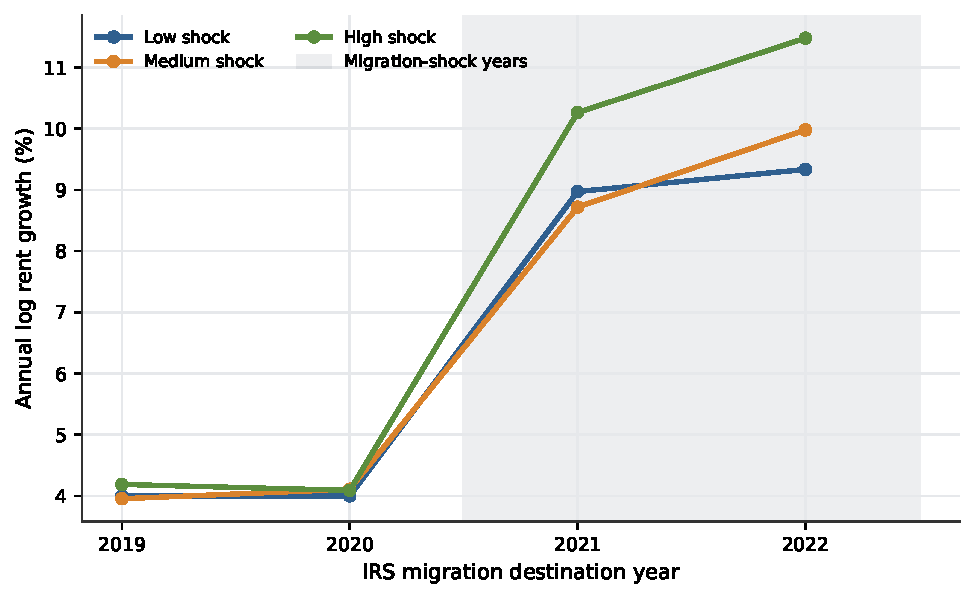
\includegraphics[width=\linewidth]{figures/iv_population_shock_timeline.pdf}
  \caption{Rent growth by migration-shock tercile}
  \label{fig:timeline}
\end{subfigure}
\hfill
\begin{subfigure}{0.49\linewidth}
  \centering
  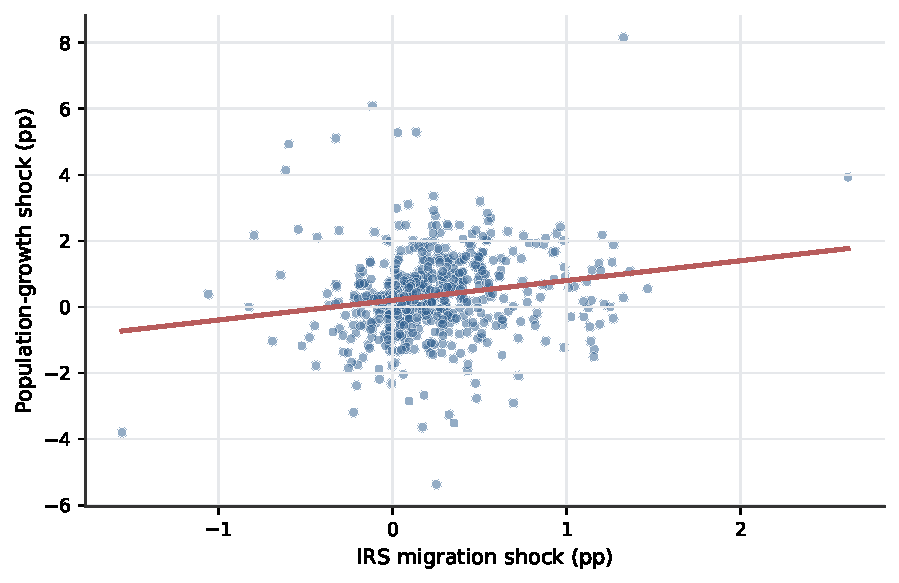
\includegraphics[width=\linewidth]{figures/iv_population_first_stage_scatter.pdf}
  \caption{First stage}
  \label{fig:firststage}
\end{subfigure}

\vspace{0.4em}
\begin{subfigure}{0.49\linewidth}
  \centering
  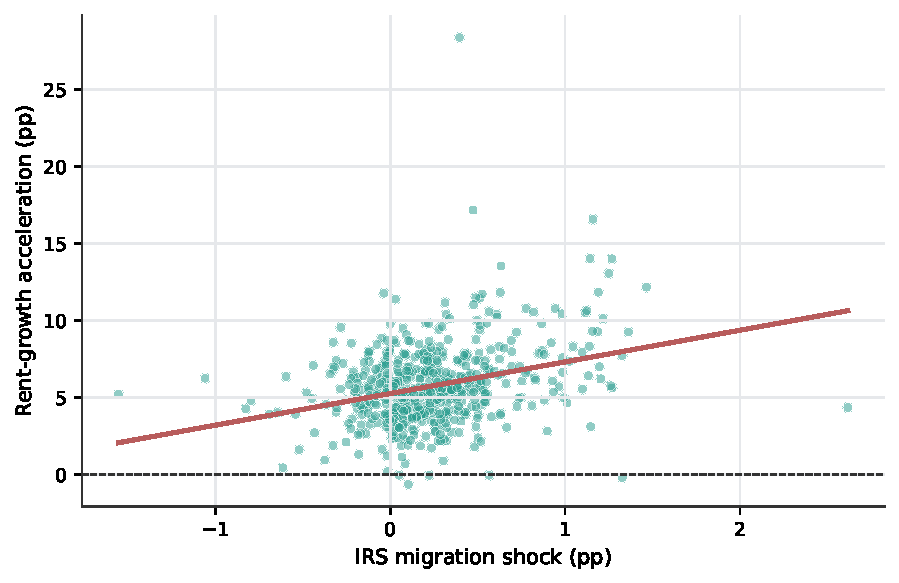
\includegraphics[width=\linewidth]{figures/iv_population_reduced_form_scatter.pdf}
  \caption{Reduced form}
  \label{fig:reducedform}
\end{subfigure}
\hfill
\begin{subfigure}{0.49\linewidth}
  \centering
  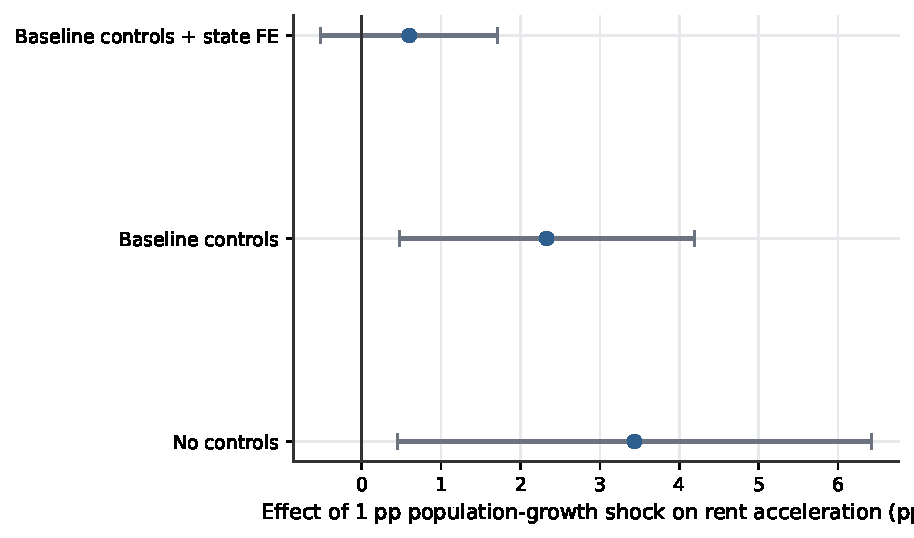
\includegraphics[width=\linewidth]{figures/iv_population_coefficient_plot.pdf}
  \caption{IV estimates}
  \label{fig:coef}
\end{subfigure}
\caption{Graphical Evidence for the IV Design}
\end{figure}

\section{Reproducibility}

The analysis is run with \texttt{analysis\_iv.py}. The merged IV datasets are saved in the \texttt{data/} folder, with regression tables in \texttt{tables/} and figures in \texttt{figures/}. The raw sources are Zillow ZORI, IRS SOI migration files, Census county population estimates, and Census Building Permits Survey files.

\begin{thebibliography}{9}

\bibitem{zillow}
Zillow Research. Housing Data: Zillow Observed Rent Index.
\url{https://www.zillow.com/research/data/}.

\bibitem{irs}
Internal Revenue Service. SOI Tax Stats - Migration Data.
\url{https://www.irs.gov/statistics/soi-tax-stats-migration-data}.

\bibitem{popest}
U.S. Census Bureau. Population and Housing Unit Estimates.
\url{https://www.census.gov/programs-surveys/popest.html}.

\bibitem{bps}
U.S. Census Bureau. Building Permits Survey.
\url{https://www.census.gov/construction/bps/}.

\end{thebibliography}

\end{document}
